\documentclass[10pt,letterpaper]{book}
\usepackage[utf8]{inputenc}
\usepackage[spanish]{babel} % varias definiciones para el español (por ejemplo usa ''Índice'' en lugar de ''Contents'')
\usepackage{hyperref}
\usepackage{geometry}
\geometry{a6paper}
% ,
%     total={210mm,297mm},
%     left=20mm,
%     right=20mm,
%     top=20mm,
%     bottom=20mm,
%     bindingoffset=0mm

\title{T\'itulo del libro}
\author{Jorge Bautista}
\begin{document}
    \frontmatter
    \maketitle
    
\chapter{Pr\'ologo}
Este es un libro que menciona de manera breve todas las caracter\'isticas del framework \href{``http://www.grails.org/''}{'Grails'} descritas en el libro \textit{``The Definitive Guide To Grails''}. No se detiene a explicar detalles. Simplemente permite que el lector se asome a la tecnolog\'ia para comenzar a conocerla o para buscar posibles soluciones a problemas encontrados durante el desarrollo.


    \mainmatter
    % \chapter{Arquitectura y comandos b\'asicos}
\chapter{Arquitectura de grails}
Grails envuelve a muchas tecnolog\'ias relacionados con \textit{java}, abstrayendo su complejidad al proporcionarnos configuraciones predeterminadas que cubren los casos de uso m\'as comunes. Estas configuraciones pueden ahorrarnos d\'ias o semanas de trabajo debido a la integraci\'on con otras tecnolog\'ias.

Aqu\'i se presentan las tecnolog\'ias principales sobre las que se Grails est\'a montado:
%En este cap\'itulo se listan las tecnolog\'ias que usa grails y comandos b\'asicos para comenzar a usarlo. 

\begin{multicols}{2}
\begin{itemize}
  \item Hibernate
  \item Spring
  \item Sitemesh
  \item Tomcat
  \item H2
  \item Groovy
  \item Gant
  \item JEE
\end{itemize}
\end{multicols}

\begin{figure}[ht!]

    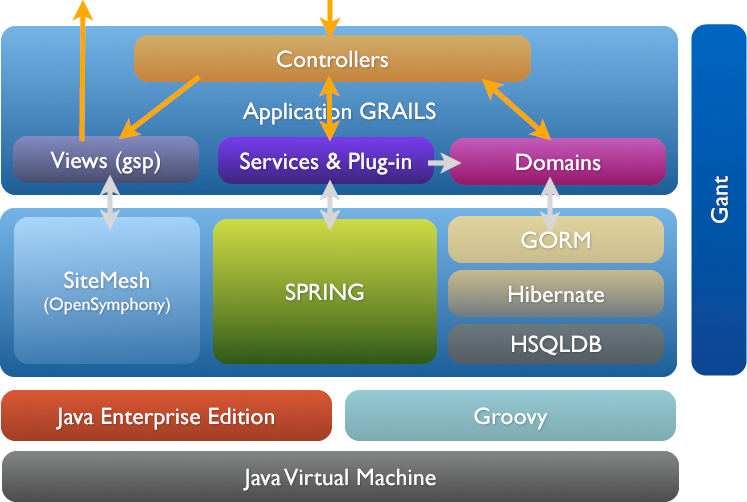
\includegraphics[width=100mm]{img/arch}
    \caption{Tecnolog\'ias que confirman la arquitectura de Grails}
    \label{arquitectura}
    

\end{figure}


    
    
    \appendix    
    \chapter{First Appendix}

    \backmatter
    \chapter{\'Ultimos comentarios}
    \nocite{*}
\end{document}

%\documentclass[a4paper,10pt]{book}
%\usepackage[utf8]{inputenc}

%\begin{document}

%\end{document}
